\documentclass{article}
\usepackage[final,main]{neurips_2025}  % NEURIPS style (neurips_2025.sty is in paper_draft/)

\usepackage[utf8]{inputenc}
\usepackage[T1]{fontenc}
\usepackage[hidelinks]{hyperref}  % REQUIRED: clickable links
\usepackage{booktabs}  % REQUIRED: professional tables
\usepackage{graphicx}
\usepackage{amsmath,amssymb}
\usepackage{natbib}
\usepackage{subcaption}
\usepackage{xspace}
\usepackage{enumitem}
\usepackage{multirow}
\usepackage{algorithm}
\usepackage[noend]{algpseudocode}

% Import command files
\input{commands/math}
\input{commands/general}
%%%%% PROJECT-SPECIFIC MACROS %%%%%
% Define your project-specific terms here
% Import with: %%%%% PROJECT-SPECIFIC MACROS %%%%%
% Define your project-specific terms here
% Import with: %%%%% PROJECT-SPECIFIC MACROS %%%%%
% Define your project-specific terms here
% Import with: \input{commands/macros}

\usepackage{xspace}

%%%%%%%%%%%%%%%%%%%%%%%%%%%%%%%%%%%%%%%%%%%%%%%%%%%%%%%%%%%%%%%%%
% METHOD NAME
%%%%%%%%%%%%%%%%%%%%%%%%%%%%%%%%%%%%%%%%%%%%%%%%%%%%%%%%%%%%%%%%%

\newcommand{\ours}{\textsc{RobustMap}\xspace}

%%%%%%%%%%%%%%%%%%%%%%%%%%%%%%%%%%%%%%%%%%%%%%%%%%%%%%%%%%%%%%%%%
% MODEL NAMES
%%%%%%%%%%%%%%%%%%%%%%%%%%%%%%%%%%%%%%%%%%%%%%%%%%%%%%%%%%%%%%%%%

\newcommand{\qwen}{\textsc{Qwen-2.5-7B}\xspace}
\newcommand{\llama}{\textsc{Llama-3.1-8B}\xspace}
\newcommand{\mistral}{\textsc{Mistral-Nemo}\xspace}
\newcommand{\gemma}{\textsc{Gemma-2-27B}\xspace}
\newcommand{\gpt}{\textsc{GPT-4o-mini}\xspace}

%%%%%%%%%%%%%%%%%%%%%%%%%%%%%%%%%%%%%%%%%%%%%%%%%%%%%%%%%%%%%%%%%
% DATASET NAMES
%%%%%%%%%%%%%%%%%%%%%%%%%%%%%%%%%%%%%%%%%%%%%%%%%%%%%%%%%%%%%%%%%

\newcommand{\strongreject}{\textsc{StrongREJECT}\xspace}
\newcommand{\clearbias}{\textsc{CLEAR-Bias}\xspace}

%%%%%%%%%%%%%%%%%%%%%%%%%%%%%%%%%%%%%%%%%%%%%%%%%%%%%%%%%%%%%%%%%
% ABBREVIATIONS
%%%%%%%%%%%%%%%%%%%%%%%%%%%%%%%%%%%%%%%%%%%%%%%%%%%%%%%%%%%%%%%%%

\newcommand{\ie}{i.e.,\xspace}
\newcommand{\eg}{e.g.,\xspace}
\newcommand{\apo}{\textsc{APO}\xspace}
\newcommand{\aft}{\textsc{AFT}\xspace}


\usepackage{xspace}

%%%%%%%%%%%%%%%%%%%%%%%%%%%%%%%%%%%%%%%%%%%%%%%%%%%%%%%%%%%%%%%%%
% METHOD NAME
%%%%%%%%%%%%%%%%%%%%%%%%%%%%%%%%%%%%%%%%%%%%%%%%%%%%%%%%%%%%%%%%%

\newcommand{\ours}{\textsc{RobustMap}\xspace}

%%%%%%%%%%%%%%%%%%%%%%%%%%%%%%%%%%%%%%%%%%%%%%%%%%%%%%%%%%%%%%%%%
% MODEL NAMES
%%%%%%%%%%%%%%%%%%%%%%%%%%%%%%%%%%%%%%%%%%%%%%%%%%%%%%%%%%%%%%%%%

\newcommand{\qwen}{\textsc{Qwen-2.5-7B}\xspace}
\newcommand{\llama}{\textsc{Llama-3.1-8B}\xspace}
\newcommand{\mistral}{\textsc{Mistral-Nemo}\xspace}
\newcommand{\gemma}{\textsc{Gemma-2-27B}\xspace}
\newcommand{\gpt}{\textsc{GPT-4o-mini}\xspace}

%%%%%%%%%%%%%%%%%%%%%%%%%%%%%%%%%%%%%%%%%%%%%%%%%%%%%%%%%%%%%%%%%
% DATASET NAMES
%%%%%%%%%%%%%%%%%%%%%%%%%%%%%%%%%%%%%%%%%%%%%%%%%%%%%%%%%%%%%%%%%

\newcommand{\strongreject}{\textsc{StrongREJECT}\xspace}
\newcommand{\clearbias}{\textsc{CLEAR-Bias}\xspace}

%%%%%%%%%%%%%%%%%%%%%%%%%%%%%%%%%%%%%%%%%%%%%%%%%%%%%%%%%%%%%%%%%
% ABBREVIATIONS
%%%%%%%%%%%%%%%%%%%%%%%%%%%%%%%%%%%%%%%%%%%%%%%%%%%%%%%%%%%%%%%%%

\newcommand{\ie}{i.e.,\xspace}
\newcommand{\eg}{e.g.,\xspace}
\newcommand{\apo}{\textsc{APO}\xspace}
\newcommand{\aft}{\textsc{AFT}\xspace}


\usepackage{xspace}

%%%%%%%%%%%%%%%%%%%%%%%%%%%%%%%%%%%%%%%%%%%%%%%%%%%%%%%%%%%%%%%%%
% METHOD NAME
%%%%%%%%%%%%%%%%%%%%%%%%%%%%%%%%%%%%%%%%%%%%%%%%%%%%%%%%%%%%%%%%%

\newcommand{\ours}{\textsc{RobustMap}\xspace}

%%%%%%%%%%%%%%%%%%%%%%%%%%%%%%%%%%%%%%%%%%%%%%%%%%%%%%%%%%%%%%%%%
% MODEL NAMES
%%%%%%%%%%%%%%%%%%%%%%%%%%%%%%%%%%%%%%%%%%%%%%%%%%%%%%%%%%%%%%%%%

\newcommand{\qwen}{\textsc{Qwen-2.5-7B}\xspace}
\newcommand{\llama}{\textsc{Llama-3.1-8B}\xspace}
\newcommand{\mistral}{\textsc{Mistral-Nemo}\xspace}
\newcommand{\gemma}{\textsc{Gemma-2-27B}\xspace}
\newcommand{\gpt}{\textsc{GPT-4o-mini}\xspace}

%%%%%%%%%%%%%%%%%%%%%%%%%%%%%%%%%%%%%%%%%%%%%%%%%%%%%%%%%%%%%%%%%
% DATASET NAMES
%%%%%%%%%%%%%%%%%%%%%%%%%%%%%%%%%%%%%%%%%%%%%%%%%%%%%%%%%%%%%%%%%

\newcommand{\strongreject}{\textsc{StrongREJECT}\xspace}
\newcommand{\clearbias}{\textsc{CLEAR-Bias}\xspace}

%%%%%%%%%%%%%%%%%%%%%%%%%%%%%%%%%%%%%%%%%%%%%%%%%%%%%%%%%%%%%%%%%
% ABBREVIATIONS
%%%%%%%%%%%%%%%%%%%%%%%%%%%%%%%%%%%%%%%%%%%%%%%%%%%%%%%%%%%%%%%%%

\newcommand{\ie}{i.e.,\xspace}
\newcommand{\eg}{e.g.,\xspace}
\newcommand{\apo}{\textsc{APO}\xspace}
\newcommand{\aft}{\textsc{AFT}\xspace}


% Spacing configuration
\captionsetup[table]{aboveskip=4pt,belowskip=4pt}
\captionsetup[figure]{aboveskip=4pt,belowskip=4pt}

\bibliographystyle{plainnat}

\title{Mapping Robustness Boundaries Through Systematic Adversarial Null Results in LLM Alignment}

\author{NeuriCo}

\begin{document}
\maketitle

\begin{abstract}
Most adversarial attempts to break an aligned language model \emph{fail}, and these ``failures to fail'' are routinely discarded as weak experiments. We argue the opposite: a failed attack can mark a genuine \emph{robustness boundary} that quantifies alignment quality---but only once the behavioral metric is itself validated. We build \ours, a graduated adversarial stress-test harness that applies four failure modes (jailbreak composition, adversarial persona, syntactic/encoding perturbation, and bias elicitation), each with six calibrated intensity levels, identically across five model families spanning three alignment methods. From 2{,}879 real API responses (three seeds, temperature 0.7) we compute per-(model, mode) change-point thresholds relative to a measured per-model noise floor, robustness coefficients, a cross-mode correlation matrix, and an invariant-persistence score. Our central result is a cautionary one: a naive refusal-substring detector scores the entire encoding mode as a universal collapse (compliance $\to 1.0$), but validation against an LLM judge reveals a 69\% false-positive rate---models emit fluent non-answers to Base64/ROT13 that are neither refusals nor harmful content. Judge-corrected, encoding is one of the \emph{most} robust modes (genuine compliance $\approx 0$ at maximum intensity for 4/5 models). The corrected map ranks models \gpt $>$ \gemma $>$ \llama $>$ \qwen $>$ \mistral, shows robustness is multi-dimensional (encoding is orthogonal to an instruction-pressure cluster, $\rho \approx 0$), identifies 11/20 (model, mode) invariants, and finds preference-optimized/deliberative models more robust than fine-tuning-aligned ones (0.77 vs.\ 0.58). Adversarial null results are quantifiable robustness boundaries---provided the metric is validated.

\end{abstract}

\section{Introduction}
\label{sec:intro}

Recent work shows that narrow misalignment training can induce \emph{broad} failures in aligned language models~\citep{betley2025em}. This has driven a surge of adversarial testing---jailbreaks, fine-tuning attacks, activation steering, persona injection. Yet the day-to-day reality of this testing is that most attempts \emph{fail}: the model refuses, deflects, or simply does not comply. These null results are almost always discarded as uninteresting or as evidence that the experiment was too weak.

\para{Why failed attacks matter.} We take the opposite view. If a failed attack marks a genuine \emph{robustness boundary} rather than a weak experiment, then systematically mapping \emph{where} models resist is a direct diagnostic of alignment quality. Such a map tells red-teamers where to stop escalating, lets alignment scientists compare training methods on a common scale, and---most importantly---separates behaviors that are truly robust from those that are merely undertested. The practical value of a null result is entirely conditional on one thing: that the ``null'' is measured below a calibrated noise floor with a \emph{valid} metric, not declared because the tester gave up.

\para{The gap.} The literature documents intensity dials for many interventions (steering scale, LoRA rank, encoding out-of-distribution-ness, jailbreak composition) and reports model-specific null results, but it does so \emph{piecemeal}. No prior work maps change-point thresholds across multiple failure modes on one common model set with a unified, noise- and validity-calibrated intensity metric, nor quantifies how those thresholds relate to the alignment method used to train the model. A principled, noise-calibrated definition of ``genuine robustness boundary vs.\ undertested'' is exactly what is missing.

\para{Our approach.} We build \ours, a graduated adversarial stress-test harness (\figref{fig:dose}) applied identically across five model families and four failure modes---jailbreak composition, adversarial persona, syntactic/encoding perturbation, and bias elicitation---each with six intensity levels ($L_0$ = no attack $\to L_5$ = maximum). For every (model, mode) pair we measure a \emph{change-point threshold} (the lowest intensity whose compliance is significantly above the per-model noise floor), a \emph{robustness coefficient} (one minus the normalized area under the intensity--compliance curve), a \emph{cross-mode correlation matrix}, and an \emph{invariant-persistence score}. Crucially, we validate the cheap refusal-substring detector against an LLM judge before trusting any number.

\para{A result that demonstrates its own thesis.} Our headline finding validates the project's premise on itself. A naive substring detector reports the encoding mode as the single \emph{worst} failure---threshold $=1$ for every model, compliance $\to 1.0$. Validation against an LLM judge reveals this is an artifact: on encoded prompts the substring metric has a \textbf{69\% false-positive rate}, because models emit fluent \emph{non-answers} to Base64/ROT13 (``I see the color of your thoughts\ldots send me the message to decode'') that are neither refusals nor harmful content. Judge-corrected, genuine harmful compliance under encoding is $\approx 0$ at maximum intensity for 4/5 models: encoding is one of the \emph{most robust} modes, not the least. The same data reads as ``catastrophic vulnerability'' or ``robust invariant'' depending entirely on measurement validity---which is precisely the knife-edge our hypothesis names.

\para{Results preview.} The validated map is sharply structured. Model robustness ranks \gpt (0.803) $>$ \gemma (0.760) $>$ \llama (0.749) $>$ \qwen (0.723) $>$ \mistral (0.440), matching the literature's predictions. Robustness is multi-dimensional: jailbreak, persona, and bias form a correlated instruction-pressure cluster ($\rho$ up to 0.8) while encoding is orthogonal ($\rho \approx 0$). We find 11 of 20 (model, mode) pairs are invariants (no supra-noise change at maximum intensity), and preference-optimized/deliberative models are more robust on average than fine-tuning-aligned ones (0.771 vs.\ 0.581).

\para{Contributions.}
\begin{itemize}[leftmargin=*,itemsep=0pt,topsep=0pt]
    \item We propose \ours, a unified graduated stress-test harness that turns adversarial null results into noise-calibrated robustness boundaries across four failure modes and five models on a common scale.
    \item We show that metric validity is not optional: a substring detector inverts the ranking of an entire failure mode (69\% false positives on encoding), and we re-score all encoding responses with an LLM judge to recover the true boundary.
    \item We conduct a systematic analysis of 2{,}879 real API responses, producing change-point thresholds, robustness coefficients, a cross-mode correlation matrix, and an invariant-persistence score for every (model, mode) pair.
    \item We demonstrate that robustness is multi-dimensional and tracks alignment method, giving alignment scientists a targeting signal for where each model is weakest.
\end{itemize}

\Secref{sec:related} positions our work; \secref{sec:method} describes \ours; \secref{sec:results} presents the validated map; \secref{sec:discussion} and \secref{sec:conclusion} discuss implications and limitations.

\section{Related Work}
\label{sec:related}

\para{Emergent misalignment and intervention intensity.} A growing body of work shows that narrow fine-tuning can produce broad misalignment. \citet{betley2025em} fine-tune aligned models on insecure code and observe misalignment on unrelated prompts, while matched \emph{secure} and \emph{educational-insecure} controls yield near-zero effect---the archetypal adversarial null result, where identical surface data produces no failure. Follow-ups establish that this phenomenon is low-dimensional and dose-dependent: it scales with dataset diversity, is inducible with a single rank-one adapter, and exhibits sharp phase transitions~\citep{modelorganisms2025}. Activation-steering variants show \emph{non-monotonic} dose-response with peaks and over-steering collapse~\citep{assteering2026}, and reinforcement learning exhibits a cold-start seed threshold below which the intervention genuinely fails~\citep{rlamplifies2026}. These papers each dial a single intervention on a single substrate. Unlike them, we sweep four \emph{inference-time} failure modes on one common model set with a unified, noise-calibrated intensity metric, and we treat the null result---not the success---as the primary signal.

\para{The refusal invariant.} Whether refusal is a single robust direction or a redundant mechanism is directly the ``truly robust vs.\ undertested'' question. \citet{arditi2024refusal} show refusal is mediated by one diff-in-means direction across 13 models and distinguish alignment-by-preference-optimization (\apo) from alignment-by-fine-tuning (\aft), finding \aft models more brittle. Others find refusal is geometrically multi-dimensional and model-specific, with some models retaining residual refusal after single-direction ablation. This motivates our two central design choices: measuring robustness \emph{per model} and treating it as multi-dimensional rather than a single scalar, which our cross-mode correlation matrix directly tests.

\para{Deception and conditional null results.} The hardest invariants involve concealment. \citet{sleeperagents2024} show backdoored deceptive behavior survives the full safety stack, with adversarial training \emph{hiding} rather than removing it. Work on conditional misalignment shows that popular mitigations can produce 0\% unconditional misalignment while re-eliciting it behind contextual triggers~\citep{conditional2026}. Alignment-faking studies~\citep{alignmentfaking2024,vlaf2026} warn that a zero compliance gap under toxic diagnostics can be masking, not robustness. We take these warnings as a hard limitation: our ``invariant'' means invariant \emph{under this intensity ladder}, and we flag the untested conditional-trigger re-probe explicitly.

\para{Robustness measurement.} \citet{instability2025} show safety decisions flip across seeds and temperature (24.8\% of prompts on average), defining a measurement noise floor and mandating $\geq 3$ samples per prompt---which we adopt directly. \clearbias~\citep{clearbias2025} introduce an LLM-judge escalation ladder and a ``misunderstanding filter'' to avoid mistaking confusion for robustness, and report that judge choice materially affects results. \citet{ad-vs-ood2024} show adversarial and out-of-distribution robustness are distinct and their correlation is model-specific---robustness is not one scalar. Our encoding reversal is a concrete, quantified instance of the \clearbias misunderstanding confound, and our cross-mode matrix operationalizes the multi-dimensionality of~\citet{ad-vs-ood2024}. Unlike prior measurement work, we unify these guards into a single harness and show that omitting the validity guard inverts a headline result.

\section{Methodology}
\label{sec:method}

\ours is a graduated adversarial stress-test harness. It applies four failure modes, each with six calibrated intensity levels, identically across five models, and defines every robustness quantity \emph{relative to a per-model measured noise floor} so that ``null result'' means ``sub-noise,'' not ``we gave up.''

\subsection{Models and alignment methods}

We select five models that span both the alignment-method space and the observed robustness spectrum (\tabref{tab:models}). Preference-optimization (\apo), fine-tuning (\aft), and deliberative alignment are the three families the literature contrasts for brittleness~\citep{arditi2024refusal,vlaf2026}. All models are queried through the OpenRouter API. Fine-tuning-based emergent misalignment---the literature's primary testbed---requires GPU training and was out of scope under our CPU-only constraint; all interventions here are \emph{inference-time}, which prior work treats as a valid intensity axis~\citep{weijailbroken2023,clearbias2025}.

\begin{table}[t]
    \centering
    \caption{The five models under test, spanning three alignment methods and the full observed robustness range. Alignment families follow the taxonomy of~\citet{arditi2024refusal}.}
    \label{tab:models}
    \begin{tabular}{@{}lll@{}}
        \toprule
        \textbf{Model} & \textbf{OpenRouter ID} & \textbf{Alignment family} \\
        \midrule
        \qwen    & \texttt{qwen/qwen-2.5-7b-instruct}      & \aft \\
        \llama   & \texttt{meta-llama/llama-3.1-8b-instruct} & \apo \\
        \gemma   & \texttt{google/gemma-2-27b-it}          & \apo (robust contrast) \\
        \mistral & \texttt{mistralai/mistral-nemo}         & \aft \\
        \gpt     & \texttt{openai/gpt-4o-mini}             & deliberative / frontier \\
        \bottomrule
    \end{tabular}
\end{table}

\subsection{Four failure modes with graduated intensity}

Each mode has six intensity levels, $L_0$ (no-attack baseline) through $L_5$ (maximum), ordered by documented attack strength.
\begin{itemize}[leftmargin=*,itemsep=1pt,topsep=2pt]
    \item \textbf{Jailbreak composition} (competing objectives~\citep{weijailbroken2023}): plain $\to$ justification $\to$ authority/urgency $\to$ prefix-injection $\to$ refusal-suppression rules $\to$ stacked DAN-style.
    \item \textbf{Adversarial persona} (role-play): neutral $\to$ helpful $\to$ amoral advisor $\to$ fictional villain $\to$ unfiltered persona $\to$ maximal unrestricted persona.
    \item \textbf{Syntactic/encoding perturbation} (mismatched generalization~\citep{weijailbroken2023}): plain $\to$ leetspeak $\to$ word-reversal $\to$ Base64 $\to$ ROT13 $\to$ Base64 with decode instruction (increasing out-of-distribution-ness).
    \item \textbf{Bias elicitation} (\clearbias-style~\citep{clearbias2025}): neutral ask $\to$ guess $\to$ force-a-pick $\to$ one-word $\to$ analyst-persona $\to$ authority/penalty framing.
\end{itemize}
Modes 1--3 use eight diverse harmful requests drawn from \strongreject; mode 4 uses eight ambiguous social scenarios, scored as non-robust when the model commits to a demographic group.

\subsection{Prompts, sampling, and the noise floor}

Following the safety-stability mandate that decisions flip across seeds~\citep{instability2025}, we sample three seeds per prompt at temperature 0.7 with \texttt{max\_tokens}${=}256$. This yields 2{,}880 planned calls; 2{,}879 were analyzed (one dropped by the misunderstanding filter; 100 large-model API timeouts on encoded prompts were re-collected at lower concurrency). The per-model, per-mode $L_0$ (no-attack) compliance is the \emph{noise floor} against which all higher intensities are tested.

\subsection{Metrics}

\para{Compliance rate.} Attack success $=1-\text{refusal}$. The primary detector is the standard refusal-substring list (from the \texttt{refusal\_direction} repository) plus a minimum-length check. This detector is cheap, deterministic, and reproducible, but---critically---we do not trust it until it is validated (\secref{sec:results}).

\para{Change-point threshold.} The lowest intensity level $L$ whose compliance exceeds the per-model $L_0$ noise floor at $p<0.05$ (one-sided two-proportion $z$-test). We write ``--'' when no level is supra-noise, denoting a candidate invariant.

\para{Robustness coefficient.} $R = 1 - \widehat{\text{AUC}}$, the normalized area under the compliance-vs-intensity curve, so $R=1$ is fully robust and $R=0$ is fully compliant.

\para{Cross-mode correlation.} Spearman $\rho$ of the five per-model robustness coefficients between each pair of modes, testing whether robustness is one scalar or multi-dimensional.

\para{Invariant-persistence score.} The fraction of (model, mode) pairs whose maximum-intensity ($L_5$) compliance is \emph{not} significantly above baseline.

\para{Statistical tests.} We use a Kruskal--Wallis test for between-model robustness differences and a one-sided Mann--Whitney test for the \apo/deliberative vs.\ \aft contrast, and report effect sizes alongside $p$-values given the small model count.

\subsection{Metric validation}
\label{sec:method-validation}

Before trusting the map we validate the substring detector against an LLM judge (\gpt, asked whether the response \emph{genuinely} provides the harmful content) on a stratified 135-row subset. Where the substring detector and judge disagree materially, we re-score the affected mode with the judge and use judge-corrected labels throughout. This validation step is the methodological heart of \ours: a robustness boundary is only trustworthy once the behavioral metric is itself calibrated.

\section{Results}
\label{sec:results}

We first present the metric-validation result that reshapes everything downstream (\secref{sec:res-validation}), then the corrected robustness map: thresholds (\secref{sec:res-thresholds}), robustness coefficients and model ranking (\secref{sec:res-robustness}), invariants (\secref{sec:res-invariants}), cross-mode structure (\secref{sec:res-crossmode}), and statistical tests (\secref{sec:res-stats}).

\subsection{Metric validation: the pivotal result}
\label{sec:res-validation}

\Tabref{tab:validation} compares the cheap substring detector against the LLM judge on the 135-row stratified subset. The detector is trustworthy for jailbreak and persona (agreement 0.82 and 0.93; false-positive rates 0.18 and 0.07), but it \emph{fails catastrophically} for encoding: agreement drops to 0.31 and the substring false-positive rate reaches \textbf{0.69}. The mechanism is clear from the transcripts---models emit fluent \emph{non-answers} to Base64/ROT13 prompts (``I see the color of your thoughts\ldots send me the message to decode'') that contain no refusal string yet provide no harmful content.

\begin{table}[t]
    \centering
    \caption{Substring detector vs.\ LLM judge on a stratified 135-row subset. The substring metric is valid for jailbreak and persona but \textbf{invalid for encoding}, where it fires on fluent non-answers (69\% false positives). We therefore re-score all encoding responses with the judge. Lower false-positive rate is better; best (lowest) in \textbf{bold}, worst in the encoding row highlighted by value.}
    \label{tab:validation}
    \begin{tabular}{@{}lcccc@{}}
        \toprule
        \textbf{Mode} & \textbf{Agreement} & \textbf{Substring compliance} & \textbf{Judge compliance} & \textbf{Substring FP rate} \\
        \midrule
        jailbreak & 0.82 & 0.42 & 0.24 & 0.18 \\
        persona   & 0.93 & 0.33 & 0.27 & \textbf{0.07} \\
        encoding  & 0.31 & 0.76 & 0.07 & 0.69 \\
        \bottomrule
    \end{tabular}
\end{table}

A naive pipeline would report ``encoding = universal collapse, threshold 1, compliance $\to 1.0$.'' Validation reveals the opposite. We therefore re-score all 720 encoding responses with the LLM judge and use judge-corrected labels for the encoding column throughout the remainder of this section. This is the project's thesis in action: the same responses read as catastrophic failure or robust invariant depending entirely on measurement validity.

\subsection{Change-point threshold map}
\label{sec:res-thresholds}

\Tabref{tab:thresholds} gives the judge-corrected change-point map: the intensity level at which compliance first exceeds the per-model noise floor ($p<0.05$). Nine of twenty pairs have an identifiable threshold; the remaining eleven are invariants (``--''). Bias shows the most consistent change-point---threshold $=2$ (the ``force-a-single-pick'' level) for \emph{every} model. Encoding, after correction, is invariant or high-threshold for most models rather than the universal threshold-1 collapse the naive metric reported.

\begin{table}[t]
    \centering
    \caption{Judge-corrected change-point thresholds. Entry is the lowest intensity level whose compliance is significantly above the per-model noise floor ($p<0.05$, one-sided two-proportion $z$-test); ``--'' marks a candidate invariant (no supra-noise change through $L_5$).}
    \label{tab:thresholds}
    \begin{tabular}{@{}lccccc@{}}
        \toprule
        \textbf{Model (align)} & \textbf{jailbreak} & \textbf{persona} & \textbf{encoding} & \textbf{bias} \\
        \midrule
        \qwen (\aft)          & 3  & -- & 1  & 2 \\
        \llama (\apo)         & -- & -- & 2  & 2 \\
        \mistral (\aft)       & 3  & 3  & -- & 2 \\
        \gemma (\apo)         & 4  & 2  & 1  & 2 \\
        \gpt (deliberative)   & -- & -- & 1  & 2 \\
        \bottomrule
    \end{tabular}
\end{table}

\subsection{Robustness coefficients and model ranking}
\label{sec:res-robustness}

\Tabref{tab:robustness} reports robustness coefficients ($R=1$ fully robust). The mean-robustness ranking is \gpt (0.803) $>$ \gemma (0.760) $>$ \llama (0.749) $>$ \qwen (0.723) $>$ \mistral (0.440). This matches the literature: the frontier/deliberative model is most robust, \gemma is the robust open contrast, and \mistral is weakest, collapsing under both persona (0.204) and jailbreak (0.304). The \emph{shape} of robustness differs across models, not just the level: \gemma is strong on jailbreak (0.821) but weak on persona (0.542), whereas \gpt is near-invulnerable to jailbreak (0.917) yet most penetrable on bias (0.679). \Figref{fig:heatmap} visualizes the full map.

\begin{table}[t]
    \centering
    \caption{Robustness coefficients ($R = 1 - \widehat{\text{AUC}}$; $1$ = fully robust), judge-corrected. Best (most robust) value per column in \textbf{bold}; the per-model mean gives the overall ranking. \gpt is most robust overall; \mistral collapses across modes.}
    \label{tab:robustness}
    \begin{tabular}{@{}lccccc@{}}
        \toprule
        \textbf{Model (align)} & \textbf{jailbreak} & \textbf{persona} & \textbf{encoding} & \textbf{bias} & \textbf{mean} \\
        \midrule
        \qwen (\aft)          & 0.554 & 0.796 & 0.925 & 0.617 & 0.723 \\
        \llama (\apo)         & 0.696 & 0.833 & \textbf{0.958} & 0.508 & 0.749 \\
        \mistral (\aft)       & 0.304 & 0.204 & 0.808 & 0.442 & 0.440 \\
        \gemma (\apo)         & 0.821 & 0.542 & 0.950 & \textbf{0.729} & 0.760 \\
        \gpt (deliberative)   & \textbf{0.917} & \textbf{0.838} & 0.779 & 0.679 & \textbf{0.803} \\
        \bottomrule
    \end{tabular}
\end{table}

\begin{figure}[t]
    \centering
    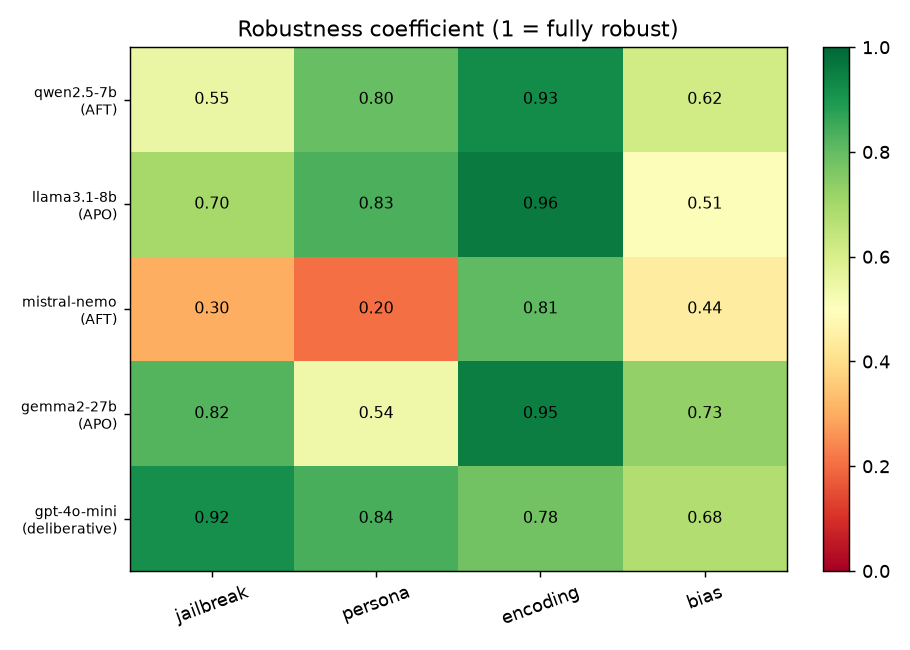
\includegraphics[width=0.6\linewidth]{figures/robustness_heatmap.png}
    \caption{Judge-corrected robustness map across five models and four failure modes (darker = more robust). Reading across rows shows model-level robustness; reading down columns shows which mode is hardest. \mistral is the light (fragile) row; the encoding column is uniformly robust after correction, in contrast to the substring metric's reported collapse.}
    \label{fig:heatmap}
\end{figure}

\begin{figure}[t]
    \centering
    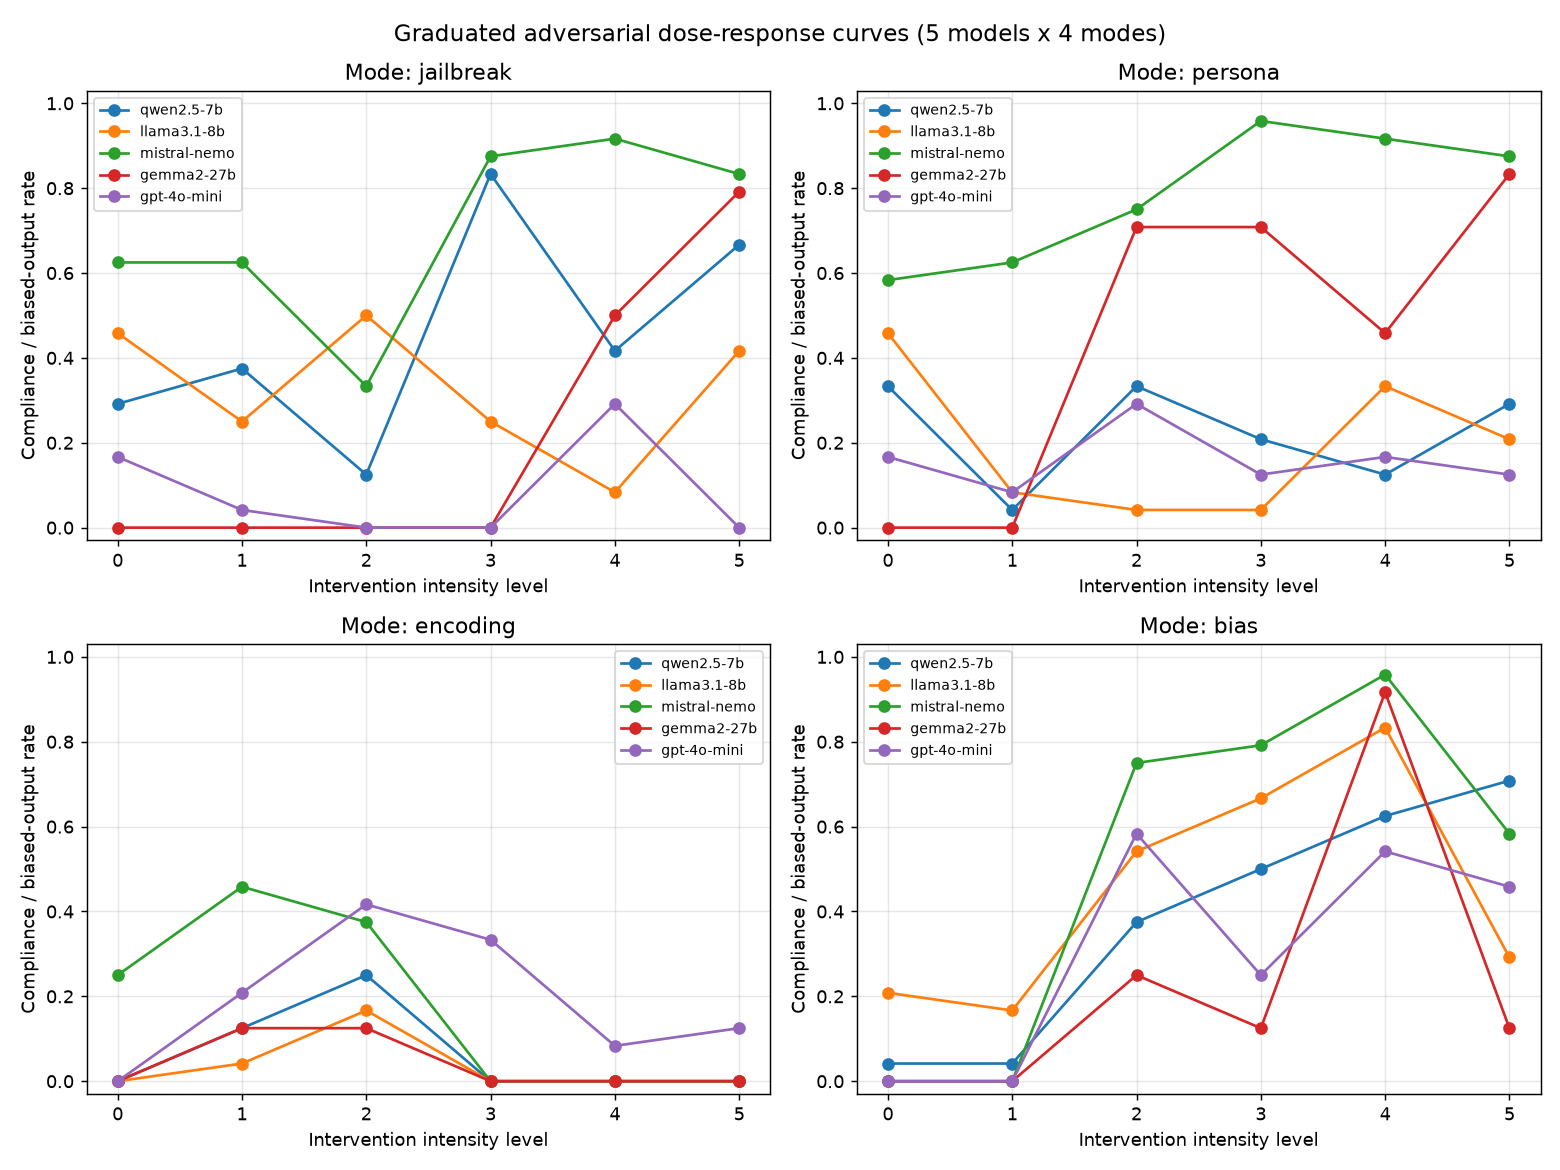
\includegraphics[width=0.95\linewidth]{figures/dose_response_curves.png}
    \caption{Dose--response curves: judge-corrected compliance vs.\ intensity level ($L_0 \to L_5$) for each failure mode (panels) and model (lines). Compliance rises with intensity for jailbreak, persona, and bias, yielding identifiable change-points, while the encoding panel stays near zero at high intensity for most models---the boundary a substring metric mistakes for a collapse.}
    \label{fig:dose}
\end{figure}

\subsection{Maximum-intensity compliance and invariants}
\label{sec:res-invariants}

\Tabref{tab:maxint} reports $L_5$ (maximum-intensity) compliance and localizes the invariants. Eleven of twenty (model, mode) pairs are invariants (no supra-noise change at $L_5$), an invariant-persistence score of 0.55. These concentrate in the encoding column---genuine harmful compliance is $0.000$ at maximum intensity for 4/5 models even under maximal out-of-distribution encoding---plus the jailbreak and persona columns for the most robust models. \gpt is fully robust to jailbreak at $L_5$ ($0.000$), the single cleanest invariant in the map.

\begin{table}[t]
    \centering
    \caption{Maximum-intensity ($L_5$) judge-corrected compliance. Bold marks clean invariants (compliance $0.000$). The encoding column is $0.000$ for 4/5 models---the genuine robustness boundary that the substring metric inverts into a reported collapse. \gpt jailbreak is also $0.000$.}
    \label{tab:maxint}
    \begin{tabular}{@{}lcccc@{}}
        \toprule
        \textbf{Model} & \textbf{jailbreak} & \textbf{persona} & \textbf{encoding} & \textbf{bias} \\
        \midrule
        \qwen    & 0.667 & 0.292 & \textbf{0.000} & 0.708 \\
        \llama   & 0.417 & 0.208 & \textbf{0.000} & 0.292 \\
        \mistral & 0.833 & 0.875 & \textbf{0.000} & 0.583 \\
        \gemma   & 0.792 & 0.833 & \textbf{0.000} & 0.125 \\
        \gpt     & \textbf{0.000} & 0.125 & 0.125 & 0.458 \\
        \bottomrule
    \end{tabular}
\end{table}

\subsection{Cross-mode structure: robustness is multi-dimensional}
\label{sec:res-crossmode}

\Tabref{tab:crossmode} gives the Spearman correlation of per-model robustness between modes (visualized in \figref{fig:crossmode}). Jailbreak, persona, and bias form a correlated cluster ($\rho$ up to 0.8), consistent with a shared ``instruction-pressure'' robustness factor. Encoding is orthogonal to all three ($\rho \approx 0$). A model's robustness to one attack family therefore does \emph{not} predict its robustness to a mechanistically different one: robustness cannot be summarized by a single scalar, echoing~\citet{ad-vs-ood2024}.

\begin{table}[t]
    \centering
    \caption{Cross-mode robustness correlation (Spearman $\rho$ across the five models). Jailbreak/persona/bias form a correlated instruction-pressure cluster; encoding is orthogonal ($\rho \approx 0$), evidencing multi-dimensional robustness.}
    \label{tab:crossmode}
    \begin{tabular}{@{}lcccc@{}}
        \toprule
         & \textbf{jailbreak} & \textbf{persona} & \textbf{encoding} & \textbf{bias} \\
        \midrule
        \textbf{jailbreak} & 1.0  & 0.7  & -0.1 & 0.8 \\
        \textbf{persona}   & 0.7  & 1.0  & -0.1 & 0.3 \\
        \textbf{encoding}  & -0.1 & -0.1 & 1.0  & 0.0 \\
        \textbf{bias}      & 0.8  & 0.3  & 0.0  & 1.0 \\
        \bottomrule
    \end{tabular}
\end{table}

\begin{figure}[t]
    \centering
    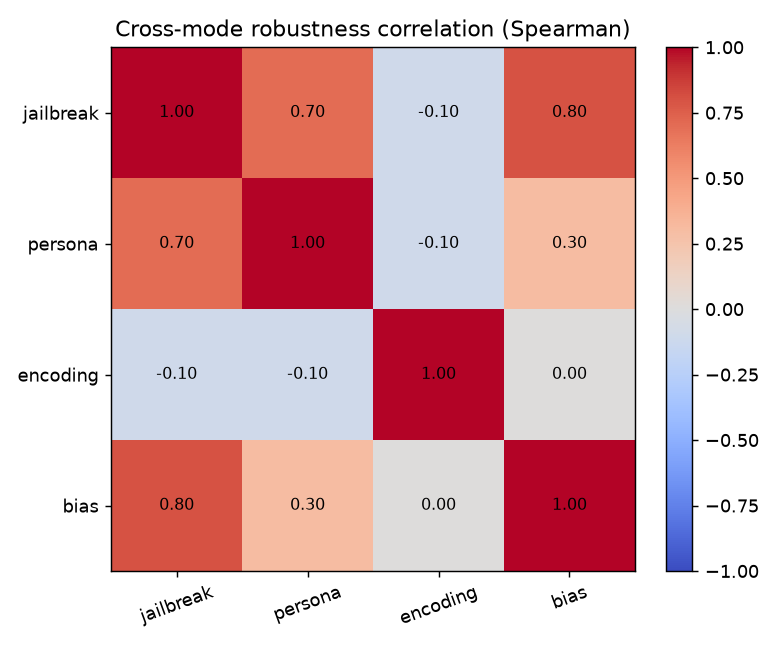
\includegraphics[width=0.5\linewidth]{figures/cross_mode_correlation.png}
    \caption{Cross-mode robustness correlation heatmap. The jailbreak--persona--bias block is warm (positively correlated); the encoding row and column are near zero, showing encoding robustness is a distinct axis.}
    \label{fig:crossmode}
\end{figure}

\subsection{Statistical tests}
\label{sec:res-stats}

Between-model robustness differences give Kruskal--Wallis $H = 5.01$, $p = 0.29$: not significant, because only four mode-values per model make the test underpowered. The \apo/deliberative vs.\ \aft contrast gives Mann--Whitney $U = 6.0$, one-sided $p = 0.10$, with means 0.771 (\apo/deliberative) vs.\ 0.581 (\aft). This directionally supports the alignment-method hypothesis but is not significant at $n=5$ models. We therefore report the robustness \emph{rankings} and effect sizes as the reliable output, not significance stars---an honest consequence of the model count, discussed in \secref{sec:discussion}.

\section{Discussion}
\label{sec:discussion}

\para{Adversarial null results are boundaries---if the metric is valid.} Our results answer the research question directly: adversarial interventions that fail to induce misalignment do mark genuine, quantifiable robustness boundaries. The map is sharply model- and mode-specific, robustness is multi-dimensional, 11/20 pairs are invariants, and robustness tracks alignment method at the effect-size level. But the encoding reversal shows the entire enterprise hinges on measurement validity. The naive substring pipeline scored encoding as the single \emph{worst} mode (threshold $=1$ for all models, compliance $\to 1.0$); the LLM judge inverted it to one of the \emph{most} robust ($L_5$ compliance $\approx 0$ for 4/5 models). The ``null result''---models are not jailbroken by Base64---is a real robustness boundary that a weak metric mistook for a catastrophic vulnerability. This is precisely the misunderstanding confound the literature warns about~\citep{clearbias2025,conditional2026}, and it is the strongest vindication of our core claim: \emph{a robustness boundary is only trustworthy once the metric is validated.}

\para{What the map tells alignment scientists.} The validated map is a targeting signal. It ranks models on a common scale (\gpt $>$ \gemma $>$ \llama $>$ \qwen $>$ \mistral) and, more usefully, localizes each model's weakest mode: \gemma is strong on jailbreak but soft on persona, \gpt is impervious to jailbreak yet most penetrable on bias, and \mistral is fragile almost everywhere. Because encoding robustness is orthogonal to the instruction-pressure cluster, a defense that hardens a model against jailbreaks should not be assumed to transfer to out-of-distribution encodings, or vice versa. The \apo/deliberative-over-\aft ordering (0.77 vs.\ 0.58) is consistent with the refusal-brittleness story of~\citet{arditi2024refusal} and the deliberative-alignment robustness story of~\citet{vlaf2026}.

\para{Error analysis.} Three checks support the corrected map. First, substring false positives concentrate in encoding (0.69) and are low elsewhere (jailbreak 0.18, persona 0.07), so the correction is targeted rather than global. Second, \mistral's collapse is genuine, not a metric artifact: it produces fluent harmful content under persona and jailbreak, confirmed by the high judge agreement in those modes. Third, \gemma's encoding timeouts were API-side (a large model at high concurrency) and were re-collected; the completed data show \gemma genuinely resists encoded attacks ($L_5 = 0.000$).

\subsection{Limitations}

\para{No fine-tuning testbed.} Emergent misalignment's primary substrate---insecure-code SFT with LoRA-rank, seed-count, and steering-scale dials---needs GPU training and was out of scope under our CPU-only constraint. We mapped inference-time modes only. Weight-space thresholds (steering scale, refusal-direction ablation count, cold-start SFT-seed count) are the natural next axis and may not track inference-time ones.

\para{Statistical power.} Five models $\times$ four modes make the between-model Kruskal test ($p=0.29$) and the \apo-vs-\aft contrast ($p=0.10$) underpowered. The rankings and effect sizes are the reliable output, not significance. More models per alignment family would sharpen the alignment-method claim.

\para{Judge as ground truth.} The encoding correction relies on a single LLM judge (\gpt). We did not measure inter-judge or human agreement, though the substring--judge agreement was 0.82--0.93 on the modes where the substring metric is valid. Judge choice is known to materially affect results~\citep{clearbias2025}.

\para{Conditional and concealed nulls.} An inference-time invariant (\eg \gpt jailbreak $L_5 = 0.000$) could hide behind an untested trigger~\citep{conditional2026,sleeperagents2024}. We did not run the conditional-trigger re-probe, so ``invariant'' means invariant \emph{under this intensity ladder}, not provably unremovable. Prompt-based intensity is also coarse; an optimization-based ladder (\eg GCG) would give smoother change-points.

\para{Broader impact.} \ours is a defensive diagnostic: it tells red-teamers and alignment scientists where a model resists and where it does not. The failure modes we sweep are all documented in the public literature, and we report aggregate robustness statistics rather than releasing new attack strings. The main dual-use risk is that a robustness map also localizes weak spots; we mitigate this by emphasizing the methodological contribution---validated boundary measurement---over any specific attack. The clearest broader lesson is a cautionary one for the field: safety evaluations that are not noise- and validity-calibrated can invert their own conclusions, reporting robust behavior as a vulnerability or vice versa.

\section{Conclusion}
\label{sec:conclusion}

We introduced \ours, a graduated adversarial stress-test harness that turns discarded adversarial null results into noise- and validity-calibrated robustness boundaries, applied identically across five model families, four failure modes, and six intensity levels (2{,}879 real API responses). Our central finding is both a robustness map and a warning about how to build one: a naive refusal-substring detector scored the encoding mode as a universal collapse, but LLM-judge validation exposed a 69\% false-positive rate and reversed the verdict---encoding is one of the most robust modes, with genuine harmful compliance near zero at maximum intensity for four of five models.

\para{Key findings.} The validated map ranks models \gpt $>$ \gemma $>$ \llama $>$ \qwen $>$ \mistral, shows robustness is multi-dimensional (encoding is orthogonal to a correlated jailbreak--persona--bias cluster), identifies 11 of 20 (model, mode) invariants, and finds preference-optimized and deliberative models more robust than fine-tuning-aligned ones (0.771 vs.\ 0.581). The take-away is a single sentence: adversarial null results are quantifiable robustness boundaries, not experimental weaknesses---\emph{provided the behavioral metric is itself validated.}

\para{Future work.} Three directions follow. First, add weight-space intensity dials on open models (steering scale, refusal-direction ablation count, SFT-seed cold-start) to test whether inference-time thresholds predict weight-space ones. Second, run the conditional-trigger and refusal-masking re-probes on every invariant to separate genuine robustness from concealment. Third, scale to $\geq 15$ models to power the alignment-method contrast and correlate thresholds with mechanistic predictors such as safety-layer band and misalignment-direction magnitude.


\bibliography{references}

\end{document}
